\documentclass[a4paper, 12pt]{article}[5.12.2012]
  \usepackage[czech]{babel}
  \usepackage[utf8]{inputenc}
  \usepackage[T1]{fontenc}
  \usepackage[text={16cm, 25cm}, left=2.5cm, top=2.5cm]{geometry}

  \usepackage{graphicx}
  \usepackage[unicode, pdfborder={0 0 0}]{hyperref}
  \usepackage{amsmath}

\begin{document}
\begin{titlepage}
\begin{center}
\textsc{{\LARGE Vysoké učení technické v Brně}\\
\smallskip
{\Large Fakulta informačních technologií}}\\
\vspace{\stretch{0.382}}
{\Large Dokumentace k projektu do předmětů IFJ a IAL}\\
\medskip
{\Huge Implementace interpretu imperativního jazyka IFJ12}\\
\vspace{\stretch{0.618}}
\end{center}
{\bf Tým 034, varianta a/1/II.}
\begin{tabbing}
Marko Fábry (vedoucí)\quad \= xfabry00\quad \= \kill
\bf{Jméno} \>  \bf{Login} \>  \bf{Rozdělení}\\
Michal Duban \> xduban01 \> 20\,\%\\
Marko Fábry (vedoucí) \> xfabry01 \> 20\,\%\\
Václav Hanselka \> xhanse00 \> 20\,\%\\
Petra Heczková \> xheczk04 \> 20\,\%\\
Jan Wrona \> xwrona00 \> 20\,\%
\end{tabbing}
\hfill \today
\end{titlepage}


\tableofcontents
\thispagestyle{empty}
\newpage
\setcounter{page}{1}
%%%%%
\section{Úvod} \label{s:uvod}
%%%%%
Tato dokumentace popisuje způsob vývoje a popis implementace interpretu imperativního jazyka
IFJ12. Projekt je rozdělen do tří základních částí: jádrem je syntaxí řízený překlad
(sekce \ref{ss:syntax}), čtení vstupního zdrojového kódu zajišťuje lexikální analyzátor
(sekce \ref{ss:lex}) a následné vykonání programu způsobuje interpret (sekce \ref{ss:interpret}).

Z řady zadání jsme si vybrali variantu a/1/II. Tato nám určila použití Knuth-Moris-Prattova 
algoritmu pro vyhledávání. Které využívá vestavěná funkce \texttt{find()}, pro vestavěnou funkci \texttt{sort()} 
bylo dle zadání nutno použít algoritmu quicksort a tabulka symbolů byla implementována pomocí hashovací tabulky.

%%%%%
\section{Popis řešení} \label{s:reseni}
%%%%%
%%%
\subsection{Lexikální analyzátor} \label{ss:lex}
%%%
Tento modul, nazvaný scanner, je jedinou částí programu operující se vstupním souborem. Jeho 
úkolem je načítání lexémů a jejich předání syntaktickému analyzátoru v podobě tokenů. 
Důležitá vlastnost je identifikace těchto lexémů, především identifikátorů, datových typů 
(číselný literál, řetězcový literál, logický literál a nil), komentářů, závorek, konců řádků apod. 
V případě identifikátoru je součástí scanneru také rozpoznání klíčových a rezervovaných slov, 
které se nesmějí použít jako identifikátor.

Implementačně je tento modul tvořen především klíčovou funkcí \texttt{GetNextToken()}, která je při 
potřebě dalšího tokenu volána z modulu syntaktického analyzátoru a předá mu strukturu 
obsahující právě jeden následující token a jeho typ. Číselný literál je načten jako řetězec, 
zkontrolován na lexikální chyby a následně převeden na datový typ double. V případě řetězcového 
literálu ohraničeného uvozovkami je implementován převod víceznakových escape sekvencí na 
jediný znak a zařazen jako součást tokenu. Při identifikaci komentáře, ať jedno čí víceřádkového, 
je zajištěno jeho přeskočení. Podstatnou funkcí je také \texttt{append()}, která počítá s předem neznámou 
délkou načítaného lexému. Tato vlastnost je zajištěna použitím knihovní funkce \texttt{realloc()}. 
Dle zadání byl scanner navrhnut a implementován jako konečný automat, jehož struktura v příloze \ref{a:fsm}.
%%%
\subsection{Syntaxí řízený překlad} \label{ss:syntax}
%%%
Syntaktický analytátor je velmi důležitý pro syntaxí řízený překlad. Zajišťuje překlad programu ve 
zdrojovém jazyce a odhalení některých druhů chyb, které se mohou při překladu objevit. Je rozdělen 
do dvou modulů, pracujících na odlišných částech kódu. S lexikálním analyzátorem komunikuje pomocí 
fuknce \texttt{GetNextToken()}.

V modulu parser je implementována metoda rekurzivního sestupu (shora dolů). Jádrem celého modulu je 
funkce \texttt{parser()}, která je volána ze souboru \texttt{ifj12.c}. Syntaktický analyzátor očekává na vstupu 
posloupnost tokenů, kontroluje jejich typ a vkládá na instruční pásku instrukce 3-adresného kódu.
Vytváří uměle funkci \texttt{main()}, kontroluje předchozí definici proměnných a jejich kolize s klíčovými 
slovy. Pokud narazí na výraz nebo příkaz výběru řetězce zavolá modul \texttt{expression}, který ho zpracuje.

Modul \texttt{expression} obsahuje globální precedenční tabulku, ve které jsou uloženy informace o prioritě 
a asociativitě operátorů. Dle zadání je použita metoda precedenční syntaktické analýzy 
(zdola nahoru). Algoritmus porovnává typ aktuálního znaku/tokenu na vstupu s typem terminálu, 
uloženým nejblíže vrcholu zásobníku (zde implementováno jako globální dynamické pole). Před vložením 
některých znaků je přidán ještě pomocný znak. Při rozhodování mezi jednotlivými pravidly se algoritmus 
řídí vzdáleností mezi pomocným znakem a vrcholem zásobníku, dále pak pro pravidlo $E\rightarrow E\ op\ E$ typem 
operátoru. Pro tento modul je zaveden nový typ tokenu \texttt{tExpression}, který označuje některé
tokeny na zásobníku. 

Funkce jsou považovány za výraz, proto se detekují v modulu \texttt{expression} kombinací proměnné 
(identifikátor funkce) a levé závorky bez operátoru mezi nimi. Podobně se detekuje i příkaz výběru řetězce. 
Mají speciální označení v precedenční tabulce. Funkce se, na rozdíl od příkazu výběru řetězce, 
dále zpracovává v modulu parser rekurzivním sestupem. Existuje několik podfunkcí zpracovávajicí několik 
variant (vestavěných) funkcí ve zdrojovém programu, např. funkce bez parametrů nebo funkce s N parametry.

Oba moduly úzce spolupracují s tabulkou symbolů. Vkládají do ní proměnné, identifikátory funkcí a uměle 
vygenerované konstanty, sloužící pro uchování mezivýpočtů. 
%%%
\subsection{Interpret} \label{ss:interpret}
%%%
Po bezchybném vykonáni syntaktické a lexikální analýzy je řízení programu předáno interpretu, 
který vykonává instrukce tříadresného kódu. Tyto instrukce jsou postupně vkládány 
syntaktickým/sémantickým analyzátorem na instrukční pásku, kterou reprezentujeme pomocí 
jednosměrně vázaného lineárního seznamu (převzat z jednoduchého interpretu)\cite{b:interpret}.

Interpret postupně prochází seznamem a vykonává příslušné instrukce. Je-li potřeba, je provedena 
kontrola správnosti typu u jednotlivých operandů (tato akce však není prováděna vždy, záleží na
konkrétní instrukci). Seznamem procházíme do té doby, dokud není nalezena instrukce \texttt{I\_STOP}, která
úspěšně ukončí interpretaci, nebo dokud není odhalena nějaká chyba. V takovém případě interpret
skončí s odpovídajícím chybovým kódem.
%%%
\subsection{Funkce \texttt{sort()}} \label{ss:sort}
%%%
Pro implementaci vestavěné funkce \texttt{sort()} jsme si vybrali zadání, které obsahuje quick\-sort, jelikož 
nám tento algoritmus byl již znám. V projektu byl použit algoritmus, který využívá rekurzi. Quicksort je možné
implementovat i pomocí cyklů, ale rekurzivní zápis se v našem případě ukázal jako vhodnější varianta.
Dále k zamyšlení byla volba pivotu a jako ideální se jevil prostřední znak řazeného řetězce či podřetězce.
Pro jednodušší pochopení algoritmu jsme využili také serveru \url{http://www.youtube.com}, kde jsme našli názornou videoukázku,
jak quicksort pracuje. 

%%%
\subsection{Funkce \texttt{find()}} \label{ss:find}
%%%
Pro implementaci vestavěné funkce \texttt{find()} jsme měli použít Knuth-Moris-Prattův algoritmus, který se 
jeví jako jednoduchý a efektivní. K pochopení KMP algoritmu stačily školní skripta. Tento algoritmus 
je výhodný, jelikož se od jakéhokoli obyčejného algoritmu liší tím že se není třeba vracet na znaky, 
které už porovnány byly a tím se proces vyhledávání zrychlí. Složitost tohoto algoritmu je $O(n+k)$.
%%%
\subsection{Tabulka symbolů}
%%%
Tabulku symbolů jsme měli podle zadání implementovat jako hashovací tabulku. Jelikož hashovací tabulka 
byla i v předmětu IAL jako domácí úloha, nebylo nutné ji znovu vymýšlet. Již napsané funkce z hashovací 
tabulky stačily jen mírně upravit, aby byla tabulka použitelná pro náš projekt. Co se týče rozptylovací 
funkce, tak tu jsme rovněž využili z předem napsané úlohy z IAL, nebylo zapotřebí ji jinak měnit, funkce 
nám vyhovovala.
%%%%%
\section{Způsob práce v týmu} \label{s:teamwork}
%%%%%
Projekt jsme nebrali na lehkou váhu, tudíž první práce začaly už v rané fázi semestru. Po konečném přihlášení
všech členů do týmu jsme uspořádali první schůzi. Jednotlivě jsme nastudovali zadání a pustili se do diskuze ohledně
nejasností, také jsme předběžně rozdělili práci mezi jednotlivé členy tak, aby rozdělení bylo rovnoměrné. Detailní
rozpis rozdělení práce je uveden v sekci \ref{ss:rozdeleni}.  Důležitým bodem na první schůzi byla také technická
stránka naší spolupráce, a to především způsob verzování, formátování a sdílení kódu, způsob vzájemné elektronické komunikace.

Nikdo z nás neměl zkušenosti s žádným VCS (version control system), ale volba nakonec padla na program git, což se ukázalo
jako dobrá volba. Ve spolupráci s teamovým privátním online repozitářem poskytovaným zdarma na serveru
\url{http://www.bitbucket.com} jsme měli k dispozici jednoduchý a spolehlivý VCS s neustálým online přístupem
ke kódu, navíc s výborným webovým grafickým rozhraním.

Co se elektronické komunikace týče, využívali jsme skupinového chatu na serveru \url{http://www.facebook.com},
ale také komunikační služby ICQ. Naší teamovou výhodou bylo ubytování všech členů na stejné koleji, proto jsme
upřednostňovali před elektronickou komunikací jednoznačně efektivnější komunikaci ústní. Také se častěji 
scházeli členové týmu, jejichž moduly spolu přímo spolupracovaly a díky tomu nebylo třeba tak často pořádat
schůze celého týmu. Přesto jsme se ale snažili každé úterý pořádat schůzi celého týmu, kde jsme
seznámili ostatní členy s důležitými změnami, které jsme během týdne provedli.
%%%
\subsection{Rozdělení práce} \label{ss:rozdeleni}
%%%
\begin{tabbing}
\texttt{expressions} \quad \= \kill
\bf{Modul} \>  \bf{Autor} \\
\texttt{expressions} \> Petra Heczková\\
\texttt{htable} \> Marko Fábry\\
\texttt{ial} \> Václav Hanselka, Marko Fábry\\
\texttt{ifj12} \> Marko Fábry\\
\texttt{ilist} \> Převzat z interpretu\cite{b:interpret} na stránkách projektu\\
\texttt{interpret} \> Michal Duban\\
\texttt{parser} \> Marko Fábry\\
\texttt{scanner} \> Jan Wrona\\
\texttt{stack} \> Marko Fábry
\end{tabbing}

%%%%%
\section{Závěr} \label{s:zaver}
%%%%%
Program byl úspěšně otestován v prostředí operačního systému Linux a to jak na serveru \texttt{merlin},
tak i na osobních počítačích s architekturami 32 i 64 bitovými. Vstupními programy pro testy byly použity
vzorové programy v zadání, naše vlastní programy, ale i kódy jiných týmu, které je zveřejnily pro testování.
Program dodržuje veškeré specifikace zadání, formát vstupních i výstupních dat, používá požadované algoritmy
a programovací techniky. Interpret může být použit jako součást dalších programů či skript, při dodržení vstupních
dat specifikovaných jazykem IFJ12.

%%%%%
\begin{thebibliography}{9}
%%%%%
\bibitem{b:honzik}
  Prof. Ing. Jan M Honzík, CSc.,
  \emph{Algoritmy: Studijní opora}.
  Verze 12-D.

\bibitem{b:meduna}
  Alexandr Meduna, Roman Lukáš,
  \emph{Formální jazyky a překladače: Studijní opora}.
  Verze 1.2006 + revize 2009 a 2010.

\bibitem{b:parser}
  \emph{Recursive descent parser}.
  In: Wikipedia: the free encyclopedia [online].
  San Francisco (CA): Wikimedia Foundation, 2001- [cit. 2012-12-09].
  Dostupné z: \url{http://en.wikipedia.org/wiki/Recursive_descent_parser}

\bibitem{b:interpret}
  \emph{Zjednodušená implementace interpretu jednoduchého jazyka}.\\
  Dostupné z: \url{https://www.fit.vutbr.cz/study/courses/IFJ/private/projekt/jednoduchy_interpret.zip}
\end{thebibliography}

%%%%%
\appendix
%%%%%
\section{Metriky kódu} \label{a:metriky}
  \paragraph{Počet souborů:} 19
  \paragraph{Počet řádků zdrojového textu:} 6135
  \paragraph{Velikost spustitelného souboru:} 63390B (systém Linux, 64 bitová
  architektura, při překladu bez ladicích informací

\section{Struktura konečného automatu} \label{a:fsm}
  \centering
  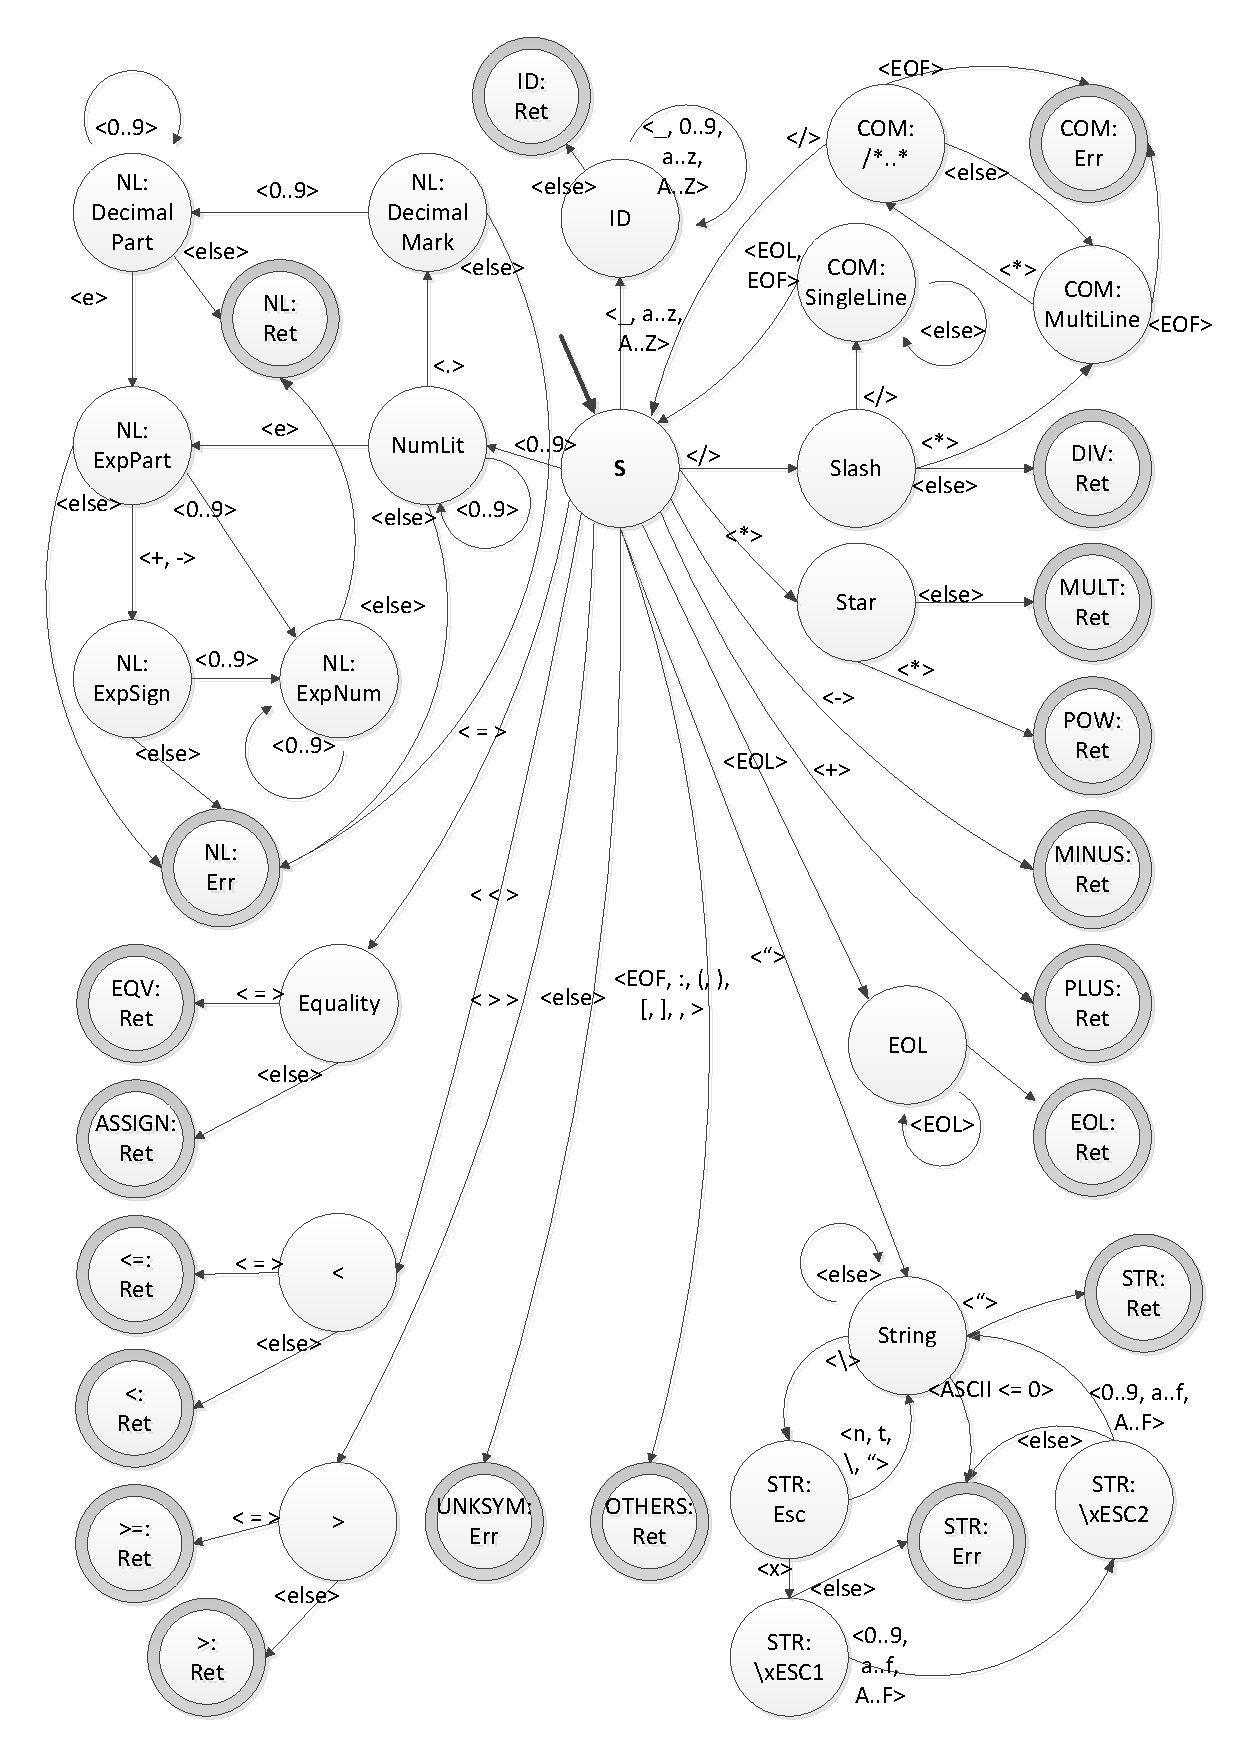
\includegraphics[scale=0.8]{fsm.pdf}

\section{LL-gramatika programových konstrukcí}
\begin{enumerate}
{\footnotesize
  \item $<program>\rightarrow<statementlist>$
  \item $<statementlist>\rightarrow<statement> <statementlist>$
  \item $<statementlist>\rightarrow<statement>$
  \item $<statement>\rightarrow \text{EOF}$
  \item $<statement>\rightarrow \text{IF} <e> \text{EOL} <statementlist> \text{ELSE EOL} <statementlist> \text{END EOL}$
  \item $<statement>\rightarrow \text{IDENT} = <e> \text{EOL}$
  \item $<statement>\rightarrow \text{IDENT} = \text{IDENT}( <arglist> \text{EOL}$
  \item $<statement>\rightarrow \text{WHILE} <e> \text{EOL} <statementList> \text{END EOL}$
  \item $<statement>\rightarrow \text{RETURN} <e> \text{EOL}$
  \item $<statement>\rightarrow \text{FUNCTION IDENT} ( <arglist> \text{EOL} <statementlist> \text{END EOL}$
  \item $<arglist>\rightarrow )$
  \item $<arglist>\rightarrow \text{IDENT} , <arglist>$
  \item $<arglist>\rightarrow \text{IDENT} )$
}
\end{enumerate}

\section{Seznam pravidel pro zpracování výrazů}
\begin{enumerate}
{\footnotesize
  \item $<e>\rightarrow \text{IDENT}$
  \item $<e>\rightarrow ( <e> )$
  \item $<e>\rightarrow<e> ** <e>$
  \item $<e>\rightarrow<e> * <e>$
  \item $<e>\rightarrow<e> / <e>$
  \item $<e>\rightarrow<e> +<e>$
  \item $<e>\rightarrow<e> -<e>$
  \item $<e>\rightarrow<e> == <e>$
  \item $<e>\rightarrow<e> \neq <e>$
  \item $<e>\rightarrow<e> \leq <e>$
  \item $<e>\rightarrow<e> \geq <e>$
  \item $<e>\rightarrow<e> < <e>$
  \item $<e>\rightarrow<e> > <e>$
  \item $<e>\rightarrow \text{IDENT} [ \text{IDENT} : \text{IDENT} ]$
}
\end{enumerate}
\end{document}
